% Evans 4.1, printed pp. 159--167; PDF pp. 176--184.
% Editorial reconstruction; independent mathematical review not performed.
\Needspace{65mm}
\section{Separation of Variables}\label{sec:4-1}
\Needspace{35mm}
\subsection{Separated modes and the missing convergence question}
For $u_t-\Delta u=0$ with zero Dirichlet data on a bounded domain $U$,
try $u(x,t)=T(t)X(x)$. On a product neighborhood where both factors
are nonzero,
\[
 \frac{T'}T=\frac{\Delta X}X=-\lambda .
\]
Fixing $x$ and then $t$ shows that the common expression is constant.
The separated equations are
\[
 -\Delta X=\lambda X,\quad X|_{\partial U}=0,\qquad
 T'=-\lambda T .
\]
The identities without division continue across zeros of $X$.
For a nonzero smooth eigenfunction, integration by parts gives
\[
 \lambda\int_U|X|^2=\int_U|DX|^2>0 .
\]
Strict positivity follows since a zero-gradient function with zero
boundary trace is zero. Thus $e^{-\lambda t}X$ is a heat mode.

\Needspace{45mm}
\PDEAnnotation{分离与叠加是两步}{乘积形式只构造单个模态；把多个模态相加依赖方程的线性。非线性方程即使能分离变量，也通常不能把分离解相加来拟合任意初值。}

\PDEBodyDiagram{4.1}{A separated mode and its nodal line.}
{On the unit square, this Dirichlet mode is the product of two one-dimensional modes. The dashed line $y=1/2$ is a zero set inside the domain. Applying $-\Delta$ adds the two eigenvalues, giving $5\pi^2$; heat evolution then changes only the time factor.}
{ch04-product-mode}

\begin{theorem}[A justified spectral representation, conditional on the spectral basis]
Assume the Dirichlet eigenfunctions $X_j$ form an orthonormal basis
of $L^2(U)$, with eigenvalues $\lambda_j>0$.
For $g\in L^2(U)$, set $g_j=(g,X_j)$ and
\[
 u(\cdot,t)=\sum_{j=1}^\infty e^{-\lambda_jt}g_jX_j .
 \tag{S4}
\]
This converges in $L^2$, tends to $g$ in $L^2$ at time zero, and
solves the heat equation in the spectral weak sense.
\end{theorem}
\begin{expandedproof}
Parseval gives $\sum|g_j|^2=\|g\|_2^2$, so the tail norm squared is
at most $\sum_{j>N}|g_j|^2$, uniformly for $t\geq0$.
Moreover
\[
 \|u(t)-g\|_2^2
 =\sum_j|e^{-\lambda_jt}-1|^2|g_j|^2\longrightarrow0
\]
by dominated convergence for a summable series.
For $t\geq\tau>0$, $\sup_{\lambda\geq0}\lambda^ke^{-\tau\lambda}<\infty$.
Hence time derivatives of every order converge in $L^2$ away from zero;
the spectral Laplacian and time derivative agree termwise.
Testing against any finite eigenfunction combination proves the weak
equation, and density extends it to the corresponding energy test class.
Interior classical smoothness requires the usual elliptic/local
regularity facts; it does not follow simply from writing (S4).
Existence and completeness of the basis are the later spectral theorem
of Chapter~6, not a conclusion of separation itself.
\end{expandedproof}
On $(0,\pi)$ one has $X_j=\sqrt{2/\pi}\sin(jx)$, $\lambda_j=j^2$.
The coefficient formula is then an ordinary sine-series expansion.
A finite sum is already a classical solution for its own initial datum.

\Needspace{35mm}
\subsection{Nonlinear and additive separation}
For $u_t-\Delta(u^m)=0$, $m>1$, try $u=T(t)X(x)\geq0$.
Homogeneity gives $T'/T^m=\Delta(X^m)/X=\mu$ and therefore
\[
 T(t)=[c-(m-1)\mu t]^{-1/(m-1)},\qquad \Delta(X^m)=\mu X .
\]
Taking $X=|x|^\alpha$ and using
$\Delta r^q=q(q+n-2)r^{q-2}$ for $r>0$ yields
\[
 \alpha=\frac2{m-1},\qquad
 \mu=\alpha m(\alpha m+n-2)>0 .
\]
The positive bracket restricts the solution interval to
$t<c/((m-1)\mu)$. At the origin $X$ need not be $C^2$,
but $X^m=r^{2+2/(m-1)}$ is $C^2$ and its Laplacian extends
continuously to zero. Thus the equation holds there in this natural
sense. The profile grows at infinity and has infinite total mass.
\Needspace{45mm}
\PDEAnnotation{无穷远的条件影响物理解}{这个分离解能在有限时间爆破，但它从一开始就有无限质量。不能用它否定有限质量、紧支集数据下的扩散结论；全空间问题也要记录增长类。}
For the Hamilton--Jacobi equation, additive separation is more natural:
$u=X(x)+T(t)$ gives $H(DX)=\mu$ and $T=-\mu t+b$.
The affine choice $X=a\cdot x$ recovers the complete family of Chapter~3.

\Needspace{35mm}
\subsection{Turing instability: diffusion can destabilize a coupled system}
Let $J=D\mathbf f(0)=\left(\begin{smallmatrix}\alpha&\beta\\
\gamma&\delta\end{smallmatrix}\right)$, and
$D=\operatorname{diag}(d_1,d_2)$, $d_i>0$.
The reaction ODE is linearly asymptotically stable precisely when
\[
 \operatorname{tr}J=\alpha+\delta<0,\qquad
 \det J=\alpha\delta-\beta\gamma>0 .
\]
Indeed its two eigenvalues either are real with negative sum and
positive product, or are conjugate with negative real part.

For $\mathbf v_t-D\Delta\mathbf v=J\mathbf v$, expand in Laplacian modes.
The coefficient of $X_j$ solves
\[
 s_j'=(J-\lambda_jD)s_j .
\]
Its trace is still negative, but its determinant is
\[
 p(\lambda)=d_1d_2\lambda^2-(d_1\delta+d_2\alpha)\lambda+\det J .
\]
\begin{theorem}[Linear mode instability]
A mode grows exponentially if and only if $p(\lambda_j)<0$.
For a continuous positive instability band it is necessary and sufficient that
\[
 B=d_1\delta+d_2\alpha>0,\qquad B^2>4d_1d_2\det J .
\]
Actual instability additionally requires a domain eigenvalue in
$(\lambda_-,\lambda_+)$, where
\[
 \lambda_\pm=\frac{B\pm\sqrt{B^2-4d_1d_2\det J}}{2d_1d_2}.
\]
\end{theorem}
\begin{expandedproof}
Negative determinant gives two real eigenvalues of opposite signs.
Positive determinant and negative trace give negative real parts;
zero determinant is a neutral threshold, not strict exponential growth.
The quadratic $p$ opens upward and has positive roots exactly under
the displayed conditions. Its negative set is the interval between them.
The discrete spectrum of the chosen domain must meet this interval.
\end{expandedproof}
\Needspace{45mm}
\PDEAnnotation{连续波段不等于域内存在模态}{代数条件先给出不稳定的 $\lambda$ 区间；还要看具体区域的离散特征值是否落入其中。$p=0$ 只是临界中性情形，严格增长需要 $p<0$。}
For example, take
\[
 J=\begin{pmatrix}1&-2\\2&-3\end{pmatrix},\qquad
 D=\operatorname{diag}(0.01,1).
\]
Then $\operatorname{tr}J=-2$, $\det J=1$, while
$p(4)=0.16-3.88+1=-2.72$.
On $(0,\pi)$ the second sine mode has $\lambda_2=4$ and grows.
If $D=dI$, by contrast, every eigenvalue is shifted by $-d\lambda_j$,
so a stable $J$ remains stable.
\Needspace{45mm}
\PDEAnnotation{线性失稳不等于已证明斑图形成}{这里证明的是线性化系统存在增长模态。非线性解是否饱和、形成何种稳定空间图案，需要额外的分岔与演化理论，不能由特征值计算直接得出。}
\par\noindent\begin{minipage}{\linewidth}
\begin{center}
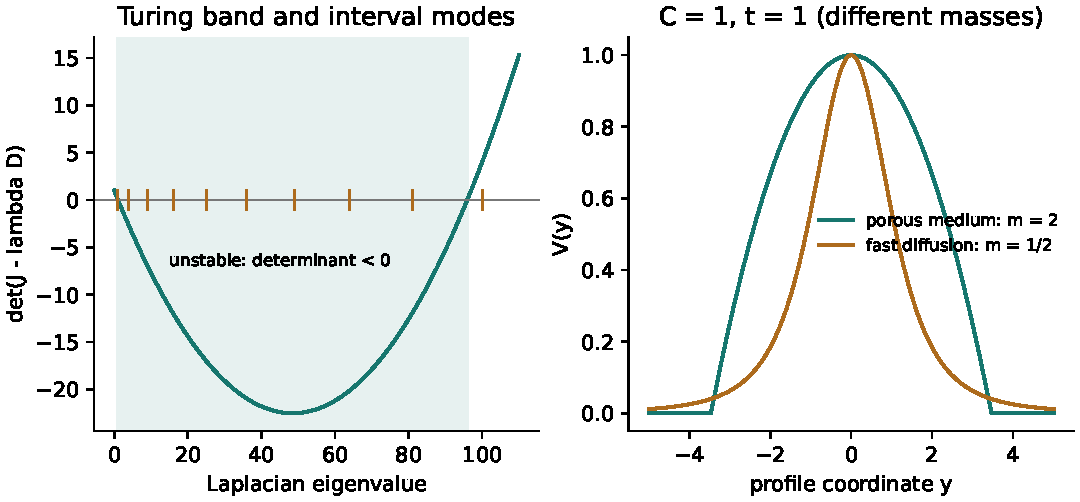
\includegraphics[width=\linewidth]{output/figures/ch04-modes-profiles.pdf}
\end{center}
\noindent\emph{Editorial figure.} The determinant band is compared with
the actual interval spectrum; the other panel compares scaling profiles.
\end{minipage}